\documentclass[aspectratio=169]{beamer}

% --- PACKAGES ---
\usepackage[utf8]{inputenc}
\usepackage[english]{babel}
\usepackage{graphicx}
\usepackage{booktabs}
\usepackage{multicol}
\usepackage{amsmath}
\usepackage{amssymb}
\usepackage{tikz}
\usetikzlibrary{positioning, arrows.meta, shapes, fit, calc}
\usepackage{pgfplots}
\pgfplotsset{compat=1.17}
\usepackage{hyperref}

% --- THEME ---
\usetheme{Madrid}
\usecolortheme{default}

% Color definitions
\definecolor{DeepBlue}{RGB}{0,51,102}
\definecolor{AlertRed}{RGB}{204,0,0}
\definecolor{SafeGreen}{RGB}{0,100,0}
\definecolor{OrangeAccent}{RGB}{230,126,34}

% --- METADATA ---
\title[Financial Networks \& Alternative Infrastructure]{Financial Networks \& Technological Innovation:\\A Dual-Network Model}

\author{Sebastián Cea \and Hernán Venegas}
\institute{Universidad de Los Andes}
\date{\today}

\begin{document}

% ===================================================================
% TITLE SLIDE
% ===================================================================
\frame{\titlepage}

% ===================================================================
% SECTION 1: MOTIVATION
% ===================================================================
\section{Motivation}

\begin{frame}{Background: Economic Impact of non Traditional Networks}

\textbf{Market Size \& Projections:}

\begin{itemize}
    \item \alert{Shadow Banking (NBFI)}: \$238.8T in assets (2023)
    \begin{itemize}
        \item[-] Now \textbf{49.1\% of global financial system} (Financial Stability Board, 2024)
    \end{itemize}
    
    \vspace{0.3cm}
    
    \item \alert{Decentralized Finance (DeFi)}: Global Decentralized Finance Market size is expected to reach \$351.75 billion by 2031
    \begin{itemize}
        \item[-] Market growth of 48.9\% CAGR (Research and Markets, 2025)
    \end{itemize}
    
    \vspace{0.3cm}
    
    \item \alert{Fintech Lending}: Tripled US mortgage market share
    \begin{itemize}
        \item[-] 14\% (2007) → 38\% (2015) (Buchak et al., 2018)
    \end{itemize}
\end{itemize}

\vspace{0.4cm}

\begin{alertblock}{Research Gap}
\centering
Theory assumes \textit{single network} but reality shows \textit{dual coexistence}\\
\textbf{Our study: a dual-network equilibrium model}
\end{alertblock}

\end{frame}

\begin{frame}{Motivating Example: Three-Agent Network}
    
    \textbf{Scenario:} National Bank, Local Bank, Local Firm
    \begin{itemize}
        \item Regulation prohibits National Bank $\leftrightarrow$ Local Firm direct lending
        \item Local Bank gets a central position
    \end{itemize}
    
    \vspace{0.5cm}
    \textbf{Impact of Restriction:}
    \begin{itemize}
        \item Bilateral volume: \textcolor{AlertRed}{-58.4\%}
        \item Aggregate welfare: \textcolor{AlertRed}{-50.8\%}
        \item Local Bank benefits (+3.8\%), endpoints lose (-84.6\%, -66.1\%)
    \end{itemize}
    
    \vspace{0.5cm}
    \textbf{Two Potential Solutions:}
    \begin{enumerate}
        \item \textbf{Competition:} Add competing central agent (Fintech)
        \item \textbf{Alternative Infrastructure:} Enable circumvention via second network
    \end{enumerate}

\end{frame}

\begin{frame}{Preview of Main Results}
    
    \textbf{Result 1: Complete Welfare Recovery via Alternative Infrastructure}
    \begin{itemize}
        \item Alternative network achieves \textcolor{SafeGreen}{\textbf{103.0\% welfare improvement}} (0.706 → 1.434)
        \item Competition alone: only 46.5\% improvement, \textcolor{AlertRed}{27.9\% gap remains}
    \end{itemize}
    
    \vspace{0.3cm}
    \textbf{Result 2: Asymmetric Adoption Despite Symmetric Networks}
    \begin{itemize}
        \item 72.4\% alternative adoption even with $\lambda_A = \tau = 0$
        \item Coexistence driven by regulations
    \end{itemize}
    
    \vspace{0.3cm}
    \textbf{Result 3: Concentrated Distributional Effects}
    \begin{itemize}
        \item Blocked party (Local Firm) captures 89.1\% of total gains
        \item Achieves utility 42.8\% \textit{above} unrestricted benchmark
    \end{itemize}
    
    \vspace{0.3cm}
    \textbf{Result 4: Friction Sensitivity}
    \begin{itemize}
        \item Operational friction ($\lambda_A$) matters 3.3× more than transparency ($\tau$)
        \item Viability requires $\lambda_A < 0.35$ even with maximal transparency
    \end{itemize}

\end{frame}

% ===================================================================
% SECTION 2: MODEL
% ===================================================================
\section{Model}

\begin{frame}{Base Framework: Jalan \& Chakrabarti (2024)}
    
    \textbf{Financial Network:} $n$ agents form bilateral contracts
    \begin{itemize}
        \item Network $W \in \mathbb{R}^{n \times n}$: $W_{ij}$ = contract size between $i$ and $j$
        \item Prices $P \in \mathbb{R}^{n \times n}$: $P_{ij} = -P_{ji}$ (zero-sum transfers)
    \end{itemize}
    
    \vspace{0.3cm}
    \textbf{Agent Characteristics:}
    \begin{itemize}
        \item Expected returns: $\mu_i \in \mathbb{R}^n$
        \item Risk aversion: $\gamma_i > 0$
        \item Covariance matrix: $\Sigma_i \succ 0$
        \item Regulatory constraints: $\Psi_i \in \{0,1\}^{n \times n}$
    \end{itemize}
    
    \vspace{0.1cm}
    \textbf{Mean-Variance Utility:}
    \begin{equation*}
    g_i(W,P) = w_i^\top (\mu_i - P e_i) - \gamma_i w_i^\top \Sigma_i w_i
    \end{equation*}
    
    \vspace{0.1cm}
    \textbf{Optimal Portfolio:} $w_i^* = Q_i(\mu_i - Pe_i)$ where $Q_i = \Psi_i^\top(2\gamma_i\Psi_i\Sigma_i\Psi_i^\top)^{-1}\Psi_i$

\end{frame}

\begin{frame}{The Dual-Network Extension}
    
    \textbf{Key Innovation: Portfolio Constraint}
    \begin{equation*}
    \boxed{w_i^* = w_i^T + w_i^A}
    \end{equation*}
    
    \begin{itemize}
        \item We set $w_i^*$ as the benchmark portfolio from the unconstrained ideal case
        \item Fixed total exposure, reallocated across networks
        \item Transforms problem into single-variable optimization
    \end{itemize}
    
    \vspace{0.3cm}
    \textbf{Network Differentiation:}
    
    \begin{enumerate}
        \item \textbf{Regulatory Treatment:} $\Psi_i^T \neq \Psi_i^A$
        \begin{itemize}
            \item Traditional: faces restrictions
            \item Alternative: permits blocked relationships ($\Psi_i^A \neq \Psi_i^T$)
        \end{itemize}
        
        \item \textbf{Friction:} $\lambda_A \geq 0$
        \begin{itemize}
            \item Quadratic cost: $\lambda_A \|w_i^A\|^2$
            \item Captures fees, congestion, integration costs
        \end{itemize}
        
        \item \textbf{Benefits:} $\tau \geq 0$
        \begin{itemize}
            \item Additive return: $+\tau \mathbf{1}$
            \item Reduced information asymmetries
        \end{itemize}
    \end{enumerate}

\end{frame}

\begin{frame}{Dual-Network Utility and Optimization}
    
    \textbf{Agent $i$'s utility decomposes across networks:}
    \begin{align*}
    g_i(w_i^T, w_i^A, P) &= g_i^T(w_i^T, P) + g_i^A(w_i^A, P)
    \end{align*}
    
    where:
    \begin{align*}
    g_i^T(w_i^T, P) &= (w_i^T)^\top(\mu_i - Pe_i) - \gamma_i (w_i^T)^\top\Sigma_i w_i^T \\
    g_i^A(w_i^A, P) &= (w_i^A)^\top(\mu_i + \tau \mathbf{1} - Pe_i) - \gamma_i (w_i^A)^\top\Sigma_i w_i^A - \lambda_A\|w_i^A\|^2
    \end{align*}
    
    \vspace{0.3cm}
    \textbf{Optimal Allocation (Proposition 1):}
    \begin{equation*}
    w_i^{T*} = Q_i^{\text{dual}} \cdot a_i
    \end{equation*}
    
    where:
    \begin{align*}
    Q_i^{\text{dual}} &= (\Psi_i^T)^\top(\Psi_i^T H_i^{-1} (\Psi_i^T)^\top)^{-1}\Psi_i^T H_i^{-1} \\
    H_i &= 2\gamma_i\Sigma_i + \lambda_A I \\
    a_i &= -\tau \mathbf{1} + (\gamma_i\Sigma_i + \lambda_A )2 w_i^*
    \end{align*}

\end{frame}

\begin{frame}{Economic Interpretation}
    
    \textbf{Cross-Network Spillovers:}
    \begin{itemize}
        \item Friction term $\lambda_A $ in $H_i = 2\gamma_i\Sigma_i + \lambda_A I$
        \item Acts as \textit{effective risk aversion increase}
        \item Alternative costs affect Traditional allocation, even for non-adopters
    \end{itemize}
    
    \vspace{0.3cm}
    \textbf{Offset Vector $a_i$ Captures:}
    \begin{itemize}
        \item Transparency benefits: $-\tau \mathbf{1}$ (pulls toward Alternative)
        \item Portfolio constraint: $(2\gamma_i\Sigma_i + 2\lambda_A I) w_i^*$ (reallocation costs)
        \item Higher friction → more Traditional allocation
    \end{itemize}
    
    \vspace{0.3cm}
    \textbf{Stability Definition:}
    
    A tuple $(W^T, W^A, P)$ is a stable point if:
    \begin{enumerate}
        \item Network symmetry: $W^T = (W^T)^\top$, $W^A = (W^A)^\top$, $P = -P^\top$
        \item Regulatory compliance: $W^T$ satisfies $\{\Psi_i^T\}$, $W^A$ satisfies $\{\Psi_i^A\}$
        \item Portfolio constraint: $w_i^T + w_i^A = w_i^*$ for all $i$
        \item Stability: Each agent maximizes utility given prices
    \end{enumerate}

\end{frame}

% ===================================================================
% SECTION 3: RESULTS
% ===================================================================
\section{Results}

\begin{frame}{Baseline Problem: Regulatory Restriction}
    
    \textbf{Three-Agent Network:} National Bank, Local Bank, Local Firm
    \begin{itemize}
        \item All agents: $\gamma_i = 1$
        \item Correlated returns: $\Sigma$ with $\rho_{13} = 0.75$
        \item \textcolor{AlertRed}{Restriction: $W_{13} = 0$ (National ↔ Local Firm blocked)}
    \end{itemize}
    
    \vspace{0.3cm}
    \begin{table}
        \centering
        \small
        \begin{tabular}{lccr}
            \toprule
            \textbf{Metric} & \textbf{Restricted} & \textbf{Unrestricted} & \textbf{Loss (\%)} \\
            \midrule
            Bilateral Volume & 0.822 & 1.976 & -58.4\% \\
            Total Utility & 0.706 & 1.434 & \textcolor{AlertRed}{-50.8\%} \\
            \midrule
            National Bank & 0.064 & 0.413 & -84.6\% \\
            Local Bank & 0.441 & 0.425 & +3.8\% \\
            Local Firm & 0.202 & 0.596 & -66.1\% \\
            \bottomrule
        \end{tabular}
    \end{table}
    
    \vspace{0.2cm}
    \textbf{Finding:} Restriction erases half of potential welfare. Local Bank benefits from structural position, endpoints suffer.

\end{frame}

\begin{frame}{Solution 1: Competition (Four Agents)}
    
    \textbf{Add Fintech:} Nearly identical to Local Bank ($\rho_{24} = 0.99$)
    
    \vspace{0.3cm}
    \begin{table}
        \centering
        \small
        \begin{tabular}{lccc}
            \toprule
            \textbf{Metric} & \textbf{Baseline} & \textbf{Competition} & \textbf{Change (\%)} \\
            & (3F-WITH) & (4F-WITH) & \\
            \midrule
            Total Utility & 0.706 & 1.034 & \textcolor{SafeGreen}{+46.5\%} \\
            Bilateral Volume & 0.822 & 1.351 & +64.3\% \\
            \midrule
            National Bank & 0.064 & 0.165 & +159.6\% \\
            Local Bank & 0.441 & 0.239 & -45.7\% \\
            Local Firm & 0.202 & 0.391 & +93.6\% \\
            Fintech & --- & 0.239 & --- \\
            \bottomrule
        \end{tabular}
    \end{table}
    
    \vspace{0.2cm}
    \textbf{Compared to Unrestricted Benchmark:}
    \begin{itemize}
        \item Competition achieves 1.034 vs. benchmark 1.434
        \item \textcolor{AlertRed}{Persistent 27.9\% welfare gap remains}
        \item Competition is \textit{second-best}, not structural solution
    \end{itemize}

\end{frame}

\begin{frame}{Solution 2: Alternative Infrastructure (Dual-Network)}
    
    \textbf{Setup:}
    \begin{itemize}
        \item Traditional: maintains restriction ($W_{13}^T = 0$)
        \item Alternative: permits all links ($\Psi_i^A = I_3$)
        \item Baseline: $\lambda_A = \tau = 0$ (no friction, no benefits)
    \end{itemize}
    
    \vspace{0.3cm}
    \begin{table}
        \centering
        \small
        \begin{tabular}{lcccc}
            \toprule
            \textbf{Metric} & \textbf{Baseline} & \textbf{Competition} & \textbf{Dual-Network} & \textbf{Benchmark} \\
             & (3F-WITH) & (4F-WITH) & (3F-DUAL) & (3F-WITHOUT) \\
            \midrule
            Total Utility & 0.706 & 1.034 & \textcolor{SafeGreen}{\textbf{1.434}} & 1.434 \\
            Gap vs. Benchmark & -50.8\% & -27.9\% & \textcolor{SafeGreen}{\textbf{0.0\%}} & 0.0\% \\
            Improvement vs. 3F-WITH & --- & +46.5\% & \textcolor{SafeGreen}{\textbf{+103.0\%}} & +103.0\% \\
            \midrule
            Bilateral Volume & 0.822 & 1.351 & 2.054 & 1.976 \\
            Direct Link $W_{13}$ & 0.000 & 0.000 & \textbf{1.033} & 1.033 \\
            \bottomrule
        \end{tabular}
    \end{table}
    
    \vspace{0.2cm}
    \textbf{Result 1:} Alternative infrastructure achieves \textcolor{SafeGreen}{\textbf{complete welfare recovery}} (100\% gap closure), while competition recovers only 46.5\%.

\end{frame}

\begin{frame}{Network Allocation: Coexistence Patterns}
    
    \textbf{Result 2: Asymmetric Adoption Despite Symmetric Networks}
    
    \vspace{0.3cm}
    \begin{columns}
        \column{0.5\textwidth}
        \begin{table}
            \centering
            \small
            \begin{tabular}{lcc}
                \toprule
                \textbf{Network} & \textbf{Volume} & \textbf{Share} \\
                \midrule
                Traditional & 0.568 & 27.6\% \\
                Alternative & 1.486 & \textcolor{SafeGreen}{\textbf{72.4\%}} \\
                \midrule
                TOTAL & 2.054 & 100\% \\
                \bottomrule
            \end{tabular}
        \end{table}
        
        \vspace{0.3cm}
        \textbf{Key Insights:}
        \begin{itemize}
            \item 72.4\% adoption with $\lambda_A = \tau = 0$
            \item Coexistence, not displacement
            \item Both networks active in equilibrium
        \end{itemize}
        
        \column{0.5\textwidth}
        \centering
        \textbf{Network Allocation}
        
        \vspace{0.5cm}
        \begin{itemize}
            \item Alternative: \textcolor{SafeGreen}{\textbf{72.4\%}}
            \item Traditional: \textcolor{DeepBlue}{27.6\%}
        \end{itemize}
        
        \vspace{0.5cm}
        \small{\textit{Regulatory arbitrage value drives adoption, not efficiency gains}}
    \end{columns}
    
    \vspace{0.3cm}
    \textbf{Mechanism:} Blocked contract ($W_{13}$) migrates entirely to Alternative, other relationships distribute across both platforms.

\end{frame}

\begin{frame}{Distributional Effects: Who Benefits?}
    
    \textbf{Result 3: Concentrated Welfare Gains}
    
    \vspace{0.3cm}
    \begin{columns}
        \column{0.55\textwidth}
        \begin{table}
            \centering
            \small
            \begin{tabular}{lcc}
                \toprule
                \textbf{Agent} & \textbf{Gain} & \textbf{\% of Total} \\
                \midrule
                Local Firm & +0.649 & \textcolor{SafeGreen}{\textbf{89.1\%}} \\
                National Bank & +0.174 & 23.9\% \\
                Local Bank & -0.096 & --- \\
                \midrule
                \textbf{TOTAL} & \textbf{+0.728} & \textbf{100\%} \\
                \bottomrule
            \end{tabular}
        \end{table}
        
        \vspace{0.3cm}
        \textbf{Utility Changes (3F-WITH → 3F-DUAL):}
        \begin{itemize}
            \item Local Firm: 0.202 → 0.851 \textcolor{SafeGreen}{(+321\%)}
            \item National Bank: 0.064 → 0.238 (+272\%)
            \item Local Bank: 0.441 → 0.345 (-21.8\%)
        \end{itemize}
        
        \column{0.45\textwidth}
        \centering
        \textbf{Welfare Distribution}
        
        \vspace{0.5cm}
        \begin{itemize}
            \item Local Firm: \textcolor{SafeGreen}{\textbf{89.1\%}}
            \item National Bank: \textcolor{DeepBlue}{23.9\%}
            \item Local Bank: \textcolor{AlertRed}{-13.0\%} (loss)
        \end{itemize}
        
        \vspace{0.5cm}
        \small{\textit{Blocked party captures majority of gains}}
        \vspace{0.2cm}
        \small{\textit{Intermediary loses structural rents}}
    \end{columns}
    
    \vspace{0.2cm}
    \textbf{Recovery:} Local Firm achieves 0.851 vs. 0.596 benchmark (+42.8\%)

\end{frame}

% ===================================================================
% SECTION 4: SENSITIVITY ANALYSIS
% ===================================================================
\section{Sensitivity Analysis}

\begin{frame}{Friction Sensitivity ($\lambda_A$)}
    
    \textbf{Result 4: Friction Dominance}
    
    \vspace{0.3cm}
    \begin{columns}
        \column{0.5\textwidth}
        \textbf{Findings ($\tau = 0$):}
        \begin{itemize}
            \item Alternative utility: 1.43 → 1.05
            \item Adoption: 50\% → 25\%
            \item \textcolor{AlertRed}{Critical threshold: $\lambda_A \approx 0.35$}
            \item Beyond threshold: <30\% adoption
        \end{itemize}
                
        \column{0.5\textwidth}
        \centering
        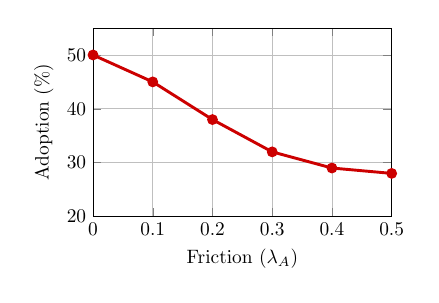
\begin{tikzpicture}[scale=0.7]
            \begin{axis}[
                xlabel={Friction ($\lambda_A$)},
                ylabel={Adoption (\%)},
                xmin=0, xmax=0.5,
                ymin=20, ymax=55,
                grid=major,
                legend pos=north east,
                width=7cm, height=5cm
            ]
            \addplot[color=AlertRed, line width=1.5pt, mark=*] coordinates {
                (0,50) (0.1,45) (0.2,38) (0.3,32) (0.4,29) (0.5,28)
            };
            \end{axis}
        \end{tikzpicture}
        
        \vspace{0.3cm}
        \small{\textit{Adoption falls nearly linearly with friction}}
    \end{columns}
    
    \vspace{0.3cm}
    \textbf{Implication:} Friction costs are significant for the alternative network viability.

\end{frame}

\begin{frame}{Benefits ($\tau$)}
    
    \textbf{Limited Compensatory Power}
    
    \vspace{0.3cm}
    \begin{columns}
        \column{0.5\textwidth}
        \textbf{Findings ($\lambda_A = 0.15$):}
        \begin{itemize}
            \item Alternative utility: 1.39 → 1.87
            \item Adoption: 37\% → 45\%
        \end{itemize}
              
        \vspace{0.3cm}
        \textbf{Relative Impact:}
        \begin{itemize}
            \item $\lambda_A$ matters 3.3× more than $\tau$
        \end{itemize}
        
        \column{0.5\textwidth}
        \centering
        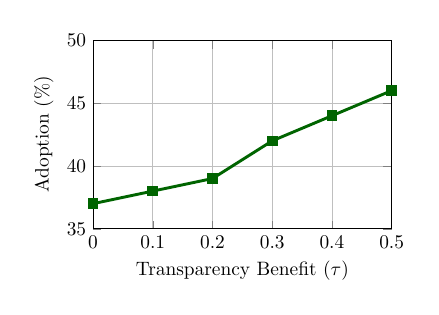
\begin{tikzpicture}[scale=0.7]
            \begin{axis}[
                xlabel={Transparency Benefit ($\tau$)},
                ylabel={Adoption (\%)},
                xmin=0, xmax=0.5,
                ymin=35, ymax=50,
                grid=major,
                legend pos=north west,
                width=7cm, height=5cm
            ]
            \addplot[color=SafeGreen, line width=1.5pt, mark=square*] coordinates {
                (0,37) (0.1,38) (0.2,39) (0.3,42) (0.4,44) (0.5,46)
            };
            \end{axis}
        \end{tikzpicture}
        
        \vspace{0.3cm}
        \small{\textit{Gradual increase, limited impact}}
    \end{columns}
    
    \vspace{0.3cm}
    \textbf{Implication:} Transparency alone cannot overcome high friction. Beyond $\lambda_A \approx 0.35$, adoption remains below 40\% even with $\tau = 0.5$.

\end{frame}

\begin{frame}{Viability Region: Joint Parameter Space}
    
    \textbf{Alternative Network Viability Conditions}
    
    \vspace{0.3cm}
    \begin{table}
        \centering
        \small
        \begin{tabular}{ccc}
            \toprule
            \textbf{Friction ($\lambda_A$)} & \textbf{Min. Transparency ($\tau$)} & \textbf{Adoption (\%)} \\
            \midrule
            0.00 & 0.00 & 50\% \\
            0.10 & 0.00 & 45\% \\
            0.20 & 0.05 & 40\% \\
            \textcolor{AlertRed}{0.35} & 0.50 & \textcolor{AlertRed}{40\%} \\
            0.50 & --- & <40\% \\
            \bottomrule
        \end{tabular}
    \end{table}
    
    \vspace{0.3cm}
    \textbf{Findings:}
    \begin{itemize}
        \item Meaningful adoption (>40\%) requires $\lambda_A < 0.35$
        \item Viable region: ~44\% of tested parameter space
        \item Coexistence plausible under relatively broad conditions
        \item Welfare recovery constant at 1.434 (portfolio constraint binding)
    \end{itemize}
    
    \vspace{0.3cm}
    \textbf{Implication:} Friction reduction more effective policy tool than transparency enhancement.

\end{frame}

% ===================================================================
% SECTION 5: POLICY IMPLICATIONS
% ===================================================================
\section{Policy Implications}

\begin{frame}{Policy Trilemma for Regulators}
    
    \textbf{When restrictions serve legitimate objectives, regulators face:}
    
    \vspace{0.3cm}
    \begin{enumerate}
        \item \textbf{Maintain Constraints}
        \begin{itemize}
            \item Preserve policy objectives (systemic risk, consumer protection)
            \item Accept 50.8\% welfare loss in our example
        \end{itemize}
        
        \vspace{0.2cm}
        \item \textbf{Prevent Circumvention}
        \begin{itemize}
            \item Block alternative infrastructure entirely
            \item Forgo 103.0\% welfare improvement
            \item May be infeasible (offshore, DeFi)
        \end{itemize}
        
        \vspace{0.2cm}
        \item \textbf{Accept Welfare Losses}
        \begin{itemize}
            \item If circumvention prevented AND constraints maintained
            \item Competition recovers only 46.5\%, persistent 27.9\% gap
        \end{itemize}
    \end{enumerate}
    
    \vspace{0.3cm}
    \begin{alertblock}{Strategic Accommodation}
    \textbf{Fourth option:} Design alternative infrastructure to minimize friction ($\lambda_A$) while maintaining oversight. Achieves welfare recovery while preserving some regulatory control.
    \end{alertblock}

\end{frame}

\begin{frame}{Competition vs. Structure}
    
    \textbf{Policy Ranking:}
    
    \vspace{0.3cm}
    \begin{table}
        \centering
        \small
        \begin{tabular}{lcc}
            \toprule
            \textbf{Policy} & \textbf{Total Utility} & \textbf{Gap Closed} \\
            \midrule
            \textcolor{SafeGreen}{\textbf{1. Remove Constraint}} & 1.434 & 100\%  \\
            \textcolor{SafeGreen}{\textbf{2. Alternative Infrastructure}} & 1.434 & 100\%  \\
            \textcolor{OrangeAccent}{3. Competition} & 1.034 & 46.5\%  \\
            \textcolor{AlertRed}{4. Baseline (Restriction)} & 0.706 & 0\% \\
            \bottomrule
        \end{tabular}
    \end{table}
    
    \vspace{0.1cm}
    \textbf{Key Insight: Infrastructure Policy > Competition Policy}
    \begin{itemize}
        \item Competition is second-best when constraints cannot be removed
        \item Only infrastructure-level solutions eliminate structural inefficiency
        \item Competition + infrastructure complementary (not substitutes)
    \end{itemize}
    
    \vspace{0.1cm}
    \textbf{Distributional Challenge:}
    \begin{itemize}
        \item 89.1\% gains to blocked party, -21.8\% to intermediary
        \item Political economy resistance from displaced incumbents
    \end{itemize}

\end{frame}

\begin{frame}{Technology Assessment Implications}
    
    \textbf{Regulatory Arbitrage vs. Efficiency}
    
    \vspace{0.3cm}
    \begin{itemize}
        \item 72.4\% adoption with $\lambda_A = \tau = 0$ (no intrinsic advantage)
        \item High adoption ≠ superior technology
        \item Adoption driven by circumvention value, not efficiency gains
    \end{itemize}
    
    \vspace{0.3cm}
    \textbf{Policy Implication:} Distinguish between:
    \begin{enumerate}
        \item \textbf{Regulatory Gap Adoption:} Driven by $\Psi_i^T \neq \Psi_i^A$
        \begin{itemize}
            \item May indicate inefficient baseline regulation
            \item Or legitimate arbitrage of socially valuable constraints
        \end{itemize}
        
        \item \textbf{Efficiency Adoption:} Driven by $\tau > 0$ or $\lambda_A < \lambda_T$
        \begin{itemize}
            \item Genuine technological improvement
            \item Should be encouraged regardless of regulation
        \end{itemize}
    \end{enumerate}
    
    \vspace{0.3cm}
    \textbf{Empirical Test:} If adoption high but $\tau \approx 0$ and $\lambda_A > 0$, regulatory arbitrage likely dominant driver.

\end{frame}

% ===================================================================
% SECTION 6: CONCLUSION
% ===================================================================
\section{Conclusion}

\begin{frame}{Contributions}
    
    \textbf{Theoretical:}
    \begin{itemize}
        \item First formal model of dual-network financial stability
        \item Portfolio constraint approach for infrastructure competition
        \item Extension of Jalan \& Chakrabarti (2024) to alternative networks
    \end{itemize}
    
    \vspace{0.3cm}
    \textbf{Empirical Calibration Potential:}
    \begin{itemize}
        \item Friction parameter ($\lambda_A$) calibrable to transaction costs
        \item Transparency parameter ($\tau$) calibrable to information asymmetries
        \item Testable predictions on adoption patterns and welfare effects
    \end{itemize}
    
    \vspace{0.3cm}
    \textbf{Policy-Relevant:}
    \begin{itemize}
        \item Quantifies limits of competition policy 
        \item Identifies critical friction threshold ($\lambda_A < 0.35$)
        \item Provides framework for strategic regulatory accommodation
    \end{itemize}

\end{frame}

\begin{frame}{Main Findings (Summary)}
    
    \begin{enumerate}
        \item \textbf{Complete Welfare Recovery via Alternative Infrastructure}
        \begin{itemize}
            \item 103.0\% improvement (0.706 → 1.434)
            \item Competition alone: only 46.5\%, persistent 27.9\% gap
        \end{itemize}
        
        \vspace{0.2cm}
        \item \textbf{Asymmetric Adoption Despite Symmetric Networks}
        \begin{itemize}
            \item 72.4\% alternative adoption with $\lambda_A = \tau = 0$
            \item Regulatory arbitrage value, not efficiency, drives adoption
        \end{itemize}
        
        \vspace{0.2cm}
        \item \textbf{Concentrated Distributional Effects}
        \begin{itemize}
            \item Blocked party captures 89.1\% of gains
            \item Recovery: 42.8\% above unrestricted benchmark
        \end{itemize}
        
        \vspace{0.2cm}
        \item \textbf{Friction Sensitivity Dominates}
        \begin{itemize}
            \item $\lambda_A$ matters 3.3× more than $\tau$
            \item Critical threshold: $\lambda_A < 0.35$ for viability
        \end{itemize}
    \end{enumerate}

\end{frame}

\begin{frame}{Limitations and Extensions}
    
    \textbf{Current Limitations:}
    \begin{itemize}
        \item Fixed total exposure ($w_i^T + w_i^A = w_i^*$)
        \item Three-agent baseline 
        \item Static stability (no transition dynamics)
    \end{itemize}
    
    \vspace{0.3cm}
    \textbf{Future Extensions:}
    \begin{enumerate}
        \item \textbf{Endogenous Exposure:} Relax portfolio constraint
        \begin{itemize}
            \item Capture expansion/contraction of total risk-taking
        \end{itemize}
        
        \item \textbf{Larger Networks:} $n > 3$ with heterogeneous intermediaries
        \begin{itemize}
            \item Richer market structure, multiple restrictions
        \end{itemize}
        
        \item \textbf{Dynamic Adoption:} Transition paths, learning effects
        \begin{itemize}
            \item Policy design for infrastructure transitions
        \end{itemize}
        
        \item \textbf{Network Externalities:} Positive feedback loops
        \begin{itemize}
            \item Multiple equilibria, path-dependence, tipping points
        \end{itemize}
    \end{enumerate}

\end{frame}

\begin{frame}
    \centering
    \Huge \textbf{Thank You}

    \vspace{0.3cm}
        
    \normalsize
    Sebastián Cea \& Hernán Venegas \\
    Universidad de Los Andes
    
    

\end{frame}

\appendix

\begin{frame}[allowframebreaks]{References}
\begin{thebibliography}{9}

\bibitem{jalan2024}
Jalan, A., \& Chakrabarti, D. (2024). 
\textit{Incentive-Aware Models of Financial Networks}. 
Operations Research, in press.

\bibitem{fsb2024}
Financial Stability Board (2024).
\textit{Global Monitoring Report on Non-Bank Financial Intermediation 2024}.

\bibitem{buchak2018}
Buchak, G., Matvos, G., Piskorski, T., \& Seru, A. (2018).
\textit{Fintech, Regulatory Arbitrage, and the Rise of Shadow Banks}.
Journal of Financial Economics, 130(3), 453-483.

\end{thebibliography}
\end{frame}

\end{document}